% \knuthc  knuth the TeXBook
% \lvoc   Lvovsky
% \lamc  lamport latex 
% \slshape different font for footnote
\graphicspath{{sec01/images/s1z/}{sec01/code/s1/}}
\lstset{inputpath=sec01/code/s1/}

\begin{frame}{What document consists of?}\relax
\begin{itemize}
    \item Title
    \item Authors
    \item Table of contents
    \item Table of figures
    \item Table of tables
    \item Sections, subsections,..
    % \item Bibliography
\end{itemize}
     
\end{frame}

%%%%%%%%%%%%%%%%%%%% Title %%%%%%%%%%%%%%%%%%%%%%
\begin{frame}[fragile]{Title}{title}\relax
\cprotect\twocolImg{
% \lstinputlisting[linerange={6-9}]{title01.tex}
\inputminted[firstline=6, lastline=9]{latex}{sec01/code/s1/title01.tex}
}{title01}
\inpause
\begin{itemize}
     \item \ccol{\title} before begin of the document
     \item \ccol{\maketitle} after begin of the document 
\end{itemize}
% \inclassFrag{Try it in your own paper!}[-1]
\skfootnote{\wikiC{https://en.wikibooks.org/wiki/LaTeX/Title_Creation} \lmanc{18.1}[163] \lmanc{8.26}[96]}
\end{frame}

\begin{frame}[fragile]{Title}{date}
 \cprotect\twocolImg{
% \lstinputlisting[linerange={6-10}]{title02.tex}
\inputminted[firstline=6, lastline=10]{latex}{sec01/code/s1/title02.tex}
}{title02}
\inpause
\begin{itemize}
     \item by defaut \LaTeX\ think you use {\csk \verb|\date{\today}|}
     \inclassFrag{what do you think command \ccol{\today} if for?}[3]
     \begin{itemize}
         \item \ccol{\today} is the date of last document compilation
     \end{itemize} 
     \inpause
     \item you can put anything inside \ccol{\date}\{\} command
     \item use \ccol{\date}\{\} without arguments to remove the string
\end{itemize}
\inpause
\inclasshigh{notice \ccol\the\ before year, month and day. We will return to it at the last lecture}
\end{frame}

\begin{frame}[fragile]{Title}{authors}
 \cprotect\twocolImg{
% \lstinputlisting[linerange={6-11}]{title03.tex}
\inputminted[firstline=6, lastline=11]{latex}{sec01/code/s1/title03.tex}
}{title03}

\inpause
\begin{itemize}
    \item \ccol\author\ for put the author
    \item \ccol\and\ (can be) used to concatinate several authors
    \begin{itemize}
        \item You always can use just plain text
    \end{itemize}
    \item \ccol\thanks\ for a footnote 
\end{itemize}
\end{frame}

\begin{frame}[fragile]{Abstract}\relax
\cprotect\twocolImg{
    \inputminted[firstline=8, lastline=10]{latex}{sec01/code/s1/abstractmy.tex}
    % \lstinputlisting[linerange={8-10}]{abstractmy.tex}
}{abstractmy}

% \inpause\inclasshigh{...Nothing happends, yeah?))}

% \outclasshigh{The style of abstract may change in specific journal, but by default there is no addition style}

\skfootnote{\lmanc{8.1}[54] \lvoc{IV.5.4}[170]}
\end{frame}

\begin{frame}[fragile]{Structure}\relax
\cprotect\twocolImg{
    \inputminted[firstline=7, lastline=15]{latex}{sec01/code/s1/struc.tex}
    % \lstinputlisting[linerange={7-15}]{struc.tex}
}{struc}

    \cprotect\skfootnote{\wikiC{https://en.wikibooks.org/wiki/LaTeX/Document_Structure\#Section_numbering}, \overC{https://www.overleaf.com/learn/latex/Sections_and_chapters}, \lmanc{6}[40], \lvoc{IV.5}[165]\\ 
    You can use \verb|\section[short name]{long name}| to put \verb|short name| to table of contents and \verb|\renewcommand{\chaptername}{new name}| (\lvoc{IV.5.3}[169]) to change the standard name
    }
\end{frame}


\begin{frame}[fragile]{Structure}{Tips}\relax

% \inclassFrag{Try \ccol\section*}[1]

\begin{itemize}
    \item Use {\csk \textbackslash<command>*} (with {\Large *}) to ommit the numbering
    \item The structure (and titles) is not pre-build into \LaTeX: they are defined inside class files $\Rightarrow$ not all classes contain all commands
     
\end{itemize}
\end{frame}

\begin{frame}[fragile]{Table of content}\relax
\cprotect\twocolImg{
    \inputminted[firstline=8, lastline=16]{latex}{sec01/code/s1/toc.tex}
    % \lstinputlisting[linerange={8-16}]{toc.tex}
}{toc}
     \inpause \ccol{\tableofcontents} for create it, \ccol{\newpage} for new page.
     
     Notice that not all structure elements are mentioned it ToC!

     \cprotect\skfootnote{\lmanc{25.1}[212]\\
     \verb|\contentsname| --- the name of the ToC; \verb|secnumdepth| counter (\lvoc{IX.3.1}[298], \lmanc{6}[40]) to change what will be included in ToC
     }
\end{frame}



\begin{frame}[fragile]{Table of...}\relax
\Large
     \begin{itemize}
          \item \ccol{\listoffigures} for figures 
          \item \ccol{\listoftables} for tables 
     \end{itemize}
     
     \cprotect\skfootnote{\lvoc{IV.8.1}[188], \lmanc{25.1}[202]\\ 
     You can use \verb|\caption[short name]{long name}| to put \verb|short name| to the lists, \verb|\listfigurename| and \verb|\listtablename| --- the names of the Lists.
     }
\end{frame}

%%%%%%%%%%%%%% IN CLASS EXERSISES
% different classes
\cprotect\inclassframe{
\begin{frame}[fragile]{\exFrame{Try to use the commands for different class files}}\relax
    \inputminted{latex}{sec01/code/s1/strucTask.tex}
    %  \lstinputlisting[linerange={1-1,7-15},basicstyle=\tt\small]{strucTask.tex}
    %  
     for {\csk book, report, article}
     
\end{frame}
}

\inclassframe{
\begin{frame}{\exFrame{Try to reproduce the following}}{lvl 1}\relax
    \begin{columns}
        \begin{column}{0.5\textwidth}
            \fbox{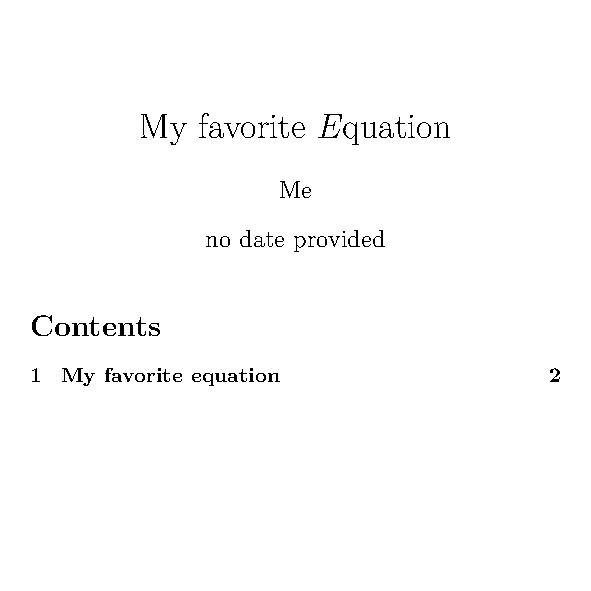
\includegraphics[height=0.7\textheight, page=1]{exStrutLvl1}}
        \end{column}
        \begin{column}{0.5\textwidth}
            \fbox{\includegraphics[height=0.7\textheight, page=2]{exStrutLvl1}}
        \end{column}
    \end{columns}
    
\end{frame}

\begin{frame}{\exFrame{Try to reproduce the following}}{lvl 2. The 2025 year must be ``current year'', not just ``2025''! \textit{You may need to google some stuff}}\relax
    
    \begin{columns}
        \begin{column}{0.5\textwidth}
            \fbox{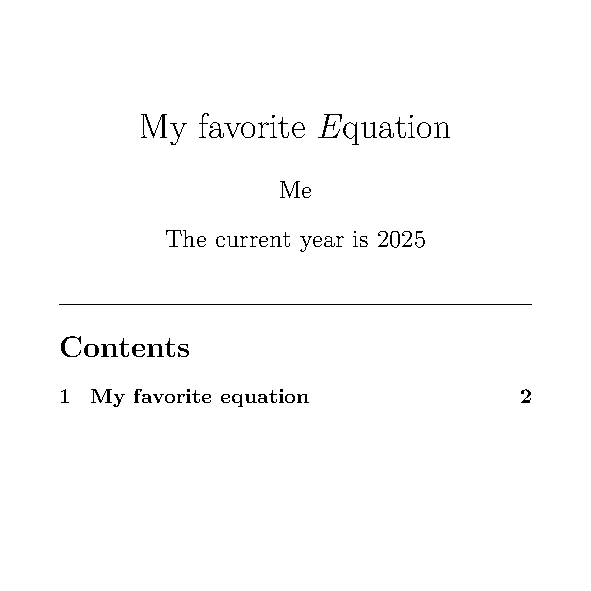
\includegraphics[height=0.7\textheight, page=1]{exStrutLvl2}}
        \end{column}
        \begin{column}{0.5\textwidth}
            \fbox{\includegraphics[height=0.7\textheight, page=2]{exStrutLvl2}}
        \end{column}
    \end{columns}
\end{frame}
}
